\chapter{Work Progress}
\label{chap:work}
\setlength{\parskip}{1.5mm}
%\setlength{\baselineskip}{1.4mm}
\section{Simulation of Non-Linear Dynamic system}
A schematic diagram of the compound triple-pendulum system is shown in Figure 5.1.The bars of the pendulum have significant mass so that it can be modeled as a compound pendulum. The model has been parameterized according to the physical characteristics of the system including mass of the bars, their inertia etc. 
% Damping factors were also included in the model for higher degree of chaos and non-linearity in the system. 
% Each bar ${i}$ is defined by a set of four parameters: 
% ${I_{i}}$, the moment of inertia of the bar, ${m_{i}}$, the mass of the bar,
%  ${L_{i}}$, the length of the bar, and
%  ${k_{i}}$, the damping coefficient of the bar rotating about it’s upper joint. 
The position and velocity of the bars are defined by the six system state variables: $\theta$\textsubscript{1}, $\theta$\textsubscript{2}, $\theta$\textsubscript{3}, ${\dot{\theta\textsubscript{1}}}$, ${\dot{\theta\textsubscript{2}}}$, ${\dot{\theta\textsubscript{3}}}$

%\begin{figure}
%\centering
%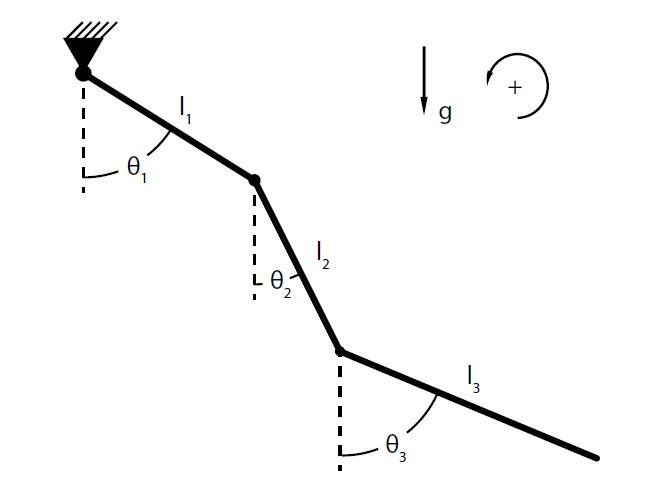
\includegraphics[width=8cm]{pendulum.jpg}
%\caption{Schematic Diagram of Triple Pendulum System}\label{fig:pendulum}
%\end{figure}
% 

\begin{figure}[H]
\begin{subfigure}{0.5\textwidth}
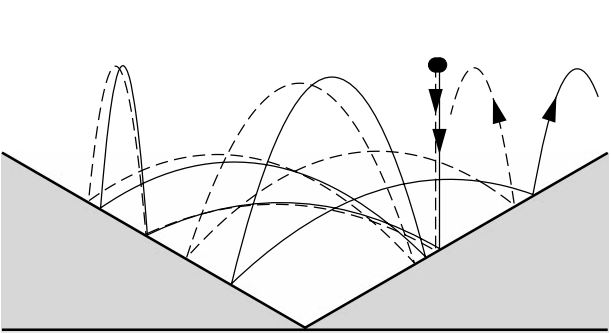
\includegraphics[width=1.1\linewidth]{ball.jpg}
\caption{Chaotic motion of a bouncing ball}\label{fig:ball}
\end{subfigure}
\begin{subfigure}{0.5\textwidth}
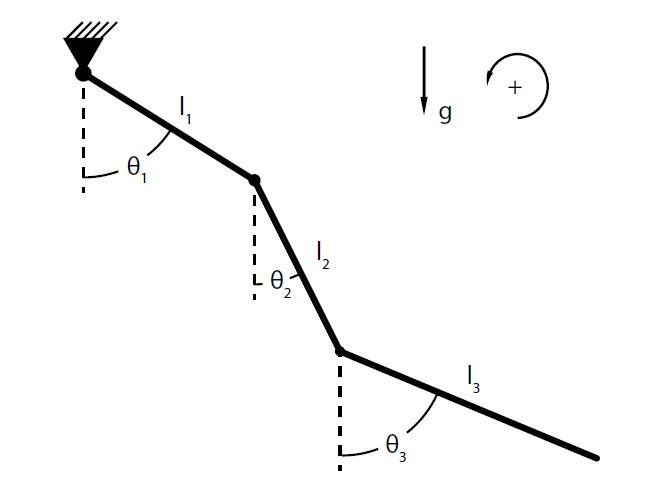
\includegraphics[width=0.8\linewidth]{pendulum.jpg}
\caption{Schematic Diagram of Triple Pendulum}\label{fig:pendulum}
\end{subfigure}
\caption{Examples of Non-Linear Dynamic systems}\label{fig:image0}

\end{figure}
\begin{figure}[h]
\begin{subfigure}{0.5\textwidth}
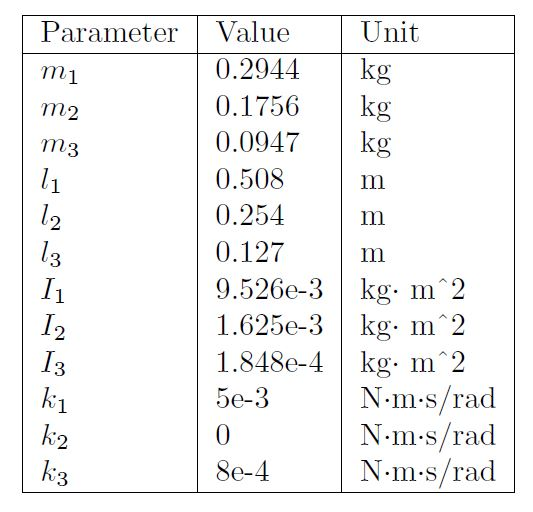
\includegraphics[width=0.8\linewidth]{param.jpg}
\caption{Table 1}\label{fig:param}
\end{subfigure}
\begin{subfigure}{0.5\textwidth}
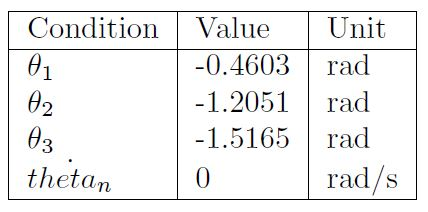
\includegraphics[width=0.8\linewidth]{ic.jpg}
\caption{Table 2}\label{fig:ic}
\end{subfigure}
\caption{Parameters \& Initial Conditions for the Initial Value Problem}\label{fig:image1}
\end{figure}

% \begin{figure}
% 
% 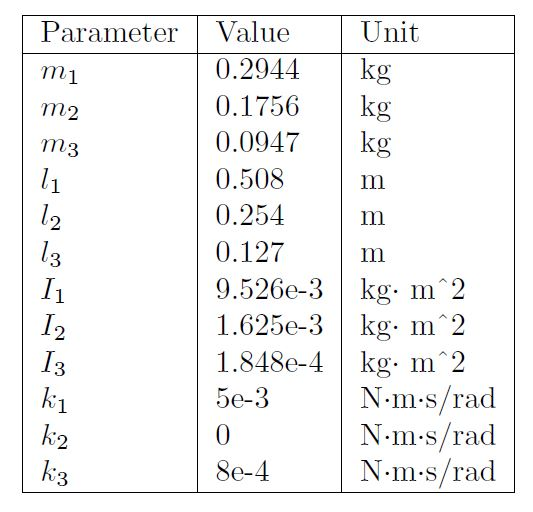
\includegraphics[width=8cm]{param.jpg}
% \caption{Parametric Values used for Simulation}\label{fig:param}
% \end{figure}
% 
% \begin{figure}
% % \centering
% 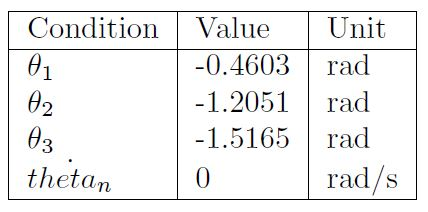
\includegraphics[width=8cm]{ic.jpg}
% \caption{Initial Conditions used for Simulation}\label{fig:ic}
% \end{figure}
\section{Verifying the scheme in MATLAB}
This compound triple-pendulum model has been simulated using MATLAB using approximate differential equations describing the random motions. The parameters and initial conditions of the ODEs are given in Table 1 and Table 2 respectively. For the simulation, simple numerical methods were used to solve the differential equations and the values corresponding to the angular position of the bars were obtained within a certain duration of time with a predefined precision. This generates the mapping values for the encryption module. 

% \begin{figure}[H]
% \centering
% 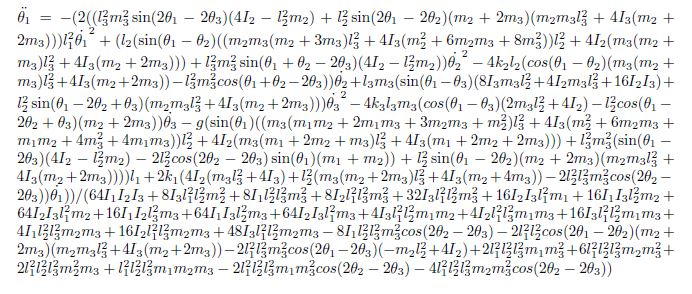
\includegraphics[width=16cm]{diff1.jpg}
% \caption{Differential Equation for ${\theta\textsubscript{1}}$}\label{fig:diff1}
% \end{figure}
% 
% 
% \begin{figure}[H]
% \centering
% 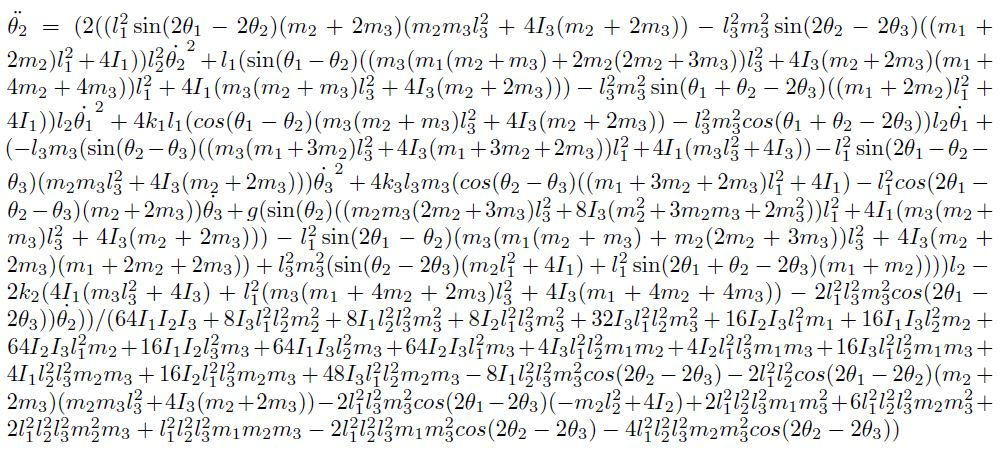
\includegraphics[width=16.5cm]{diff2.jpg}
% \caption{Differential Equation for ${\theta\textsubscript{2}}$}\label{fig:diff2}
% \end{figure}
% 
% 
% \begin{figure}[H]
% \centering
% 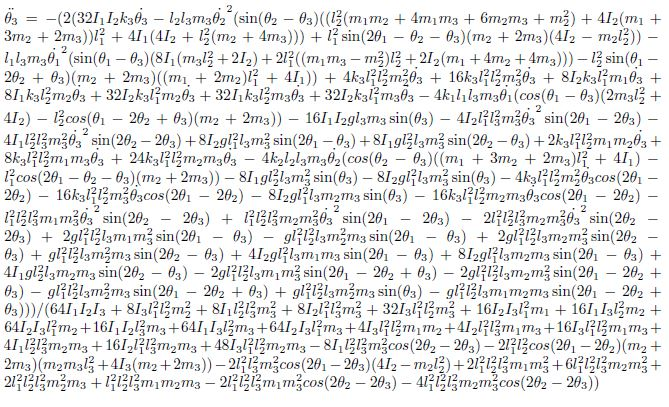
\includegraphics[width=16.5cm]{diff3.jpg}
% \caption{Differential Equation for ${\theta\textsubscript{3}}$}\label{fig:diff3}
% \end{figure}
% \vfill
\subsection{Simulation Results}
These are some of the observations from the simulation of the triple-pendulum model for a duration of t = 0 to t = 20 seconds :\\
(i) Initial conditions are same as given in Table 1 \& 2:\\
 
\begin{figure}[H]
\begin{subfigure}{0.5\textwidth}
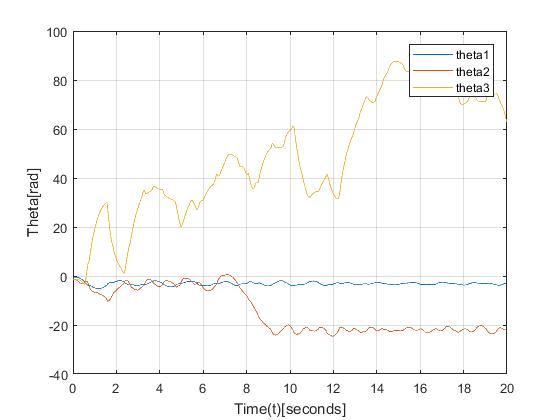
\includegraphics[width=1\linewidth]{s1.jpg}
\caption{Plot of ${\theta}$ vs Time}\label{fig:s1}
\end{subfigure}
\begin{subfigure}{0.5\textwidth}
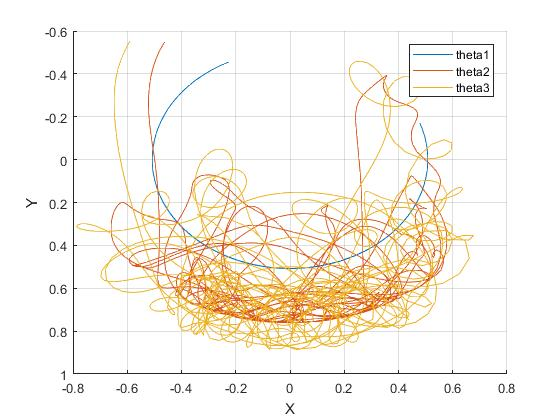
\includegraphics[width=1\linewidth]{path1.jpg}
\caption{Plot of Motion of Triple-Pendulum}\label{fig:path1}
\end{subfigure}
\caption{Motion of Triple-Pendulum for t = 0 to t = 20 sec}\label{fig:image2}
\end{figure}

\begin{figure}[H]
\centering
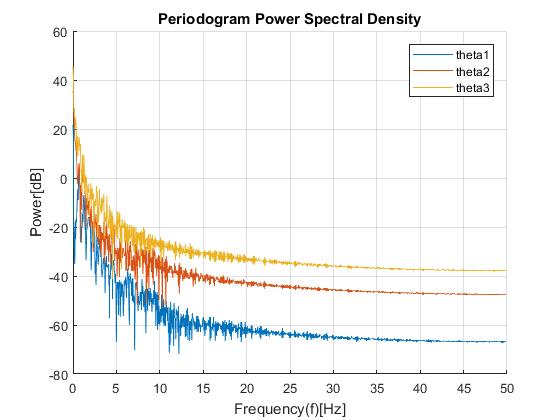
\includegraphics[width=10cm]{p1.jpg}
\caption{Periodogram Plot for ${\theta}$ }\label{fig:p1}
\end{figure}

\begin{figure}[H]
\begin{subfigure}{0.5\textwidth}
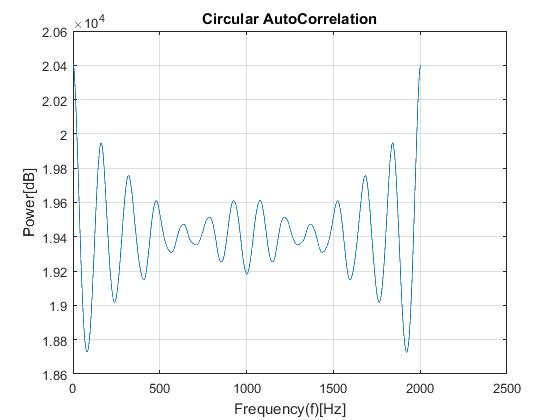
\includegraphics[width=1\linewidth]{cirauto1.jpg}
\caption{Plot of Circular Auto-Correlation for ${\theta_{1}}$}\label{fig:cirauto1}
\end{subfigure}
\begin{subfigure}{0.5\textwidth}
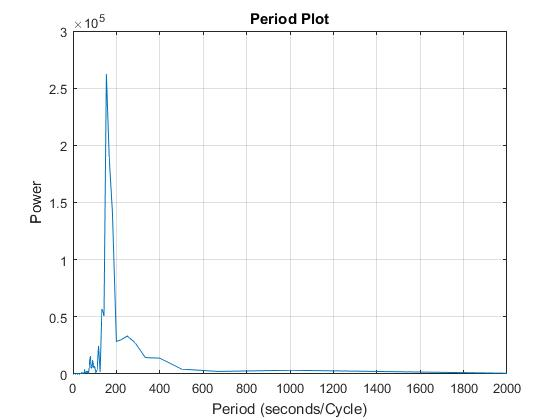
\includegraphics[width=1\linewidth]{pp1.jpg}
\caption{Plot of Periodicity for ${\theta_{1}}$}\label{fig:pp1}
\end{subfigure}
\caption{Periodic Properties of ${\theta_{1}}$}\label{fig:image3}
\end{figure}



It is observed that for certain specific parameters or initial conditions, the motion of the bars of the triple-pendulum shows periodic nature after a certain span of time. Hence there is a need to eliminate those parameters or initial conditions for which the motion is periodic as the periodic nature breaks the chaotic behavior of the system. For that a test for periodicity was employed to extract the prominent period of the signal using statistical analysis on the spectrum of the signal. The test used is known as {\bf{\em Fisher's g-statistic test}}. This method is based on the test of significance of the periodic components of the signal derived from its periodogram. 

These are some of the observations from the simulation of the triple-pendulum model for a duration of t = 0 to t = 10 seconds :\\
(i) Initial conditions are same as given in Table 1 \& 2 with ${l_{2}}$ = 0.381 m and ${l_{3}}$ = 1.143m :\\

\begin{figure}[H]
\begin{subfigure}{0.5\textwidth}
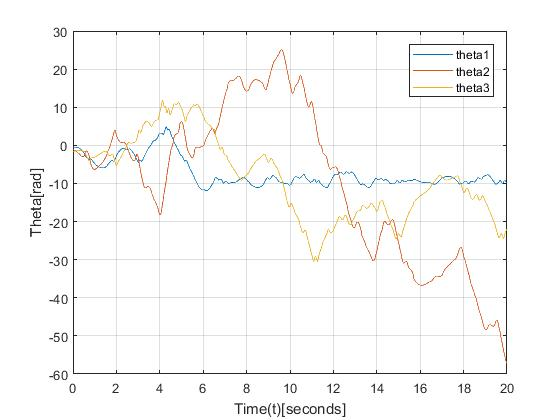
\includegraphics[width=1\linewidth]{s2.jpg}
\caption{Plot of ${\theta}$ vs Time}\label{fig:s2}
\end{subfigure}
\begin{subfigure}{0.5\textwidth}
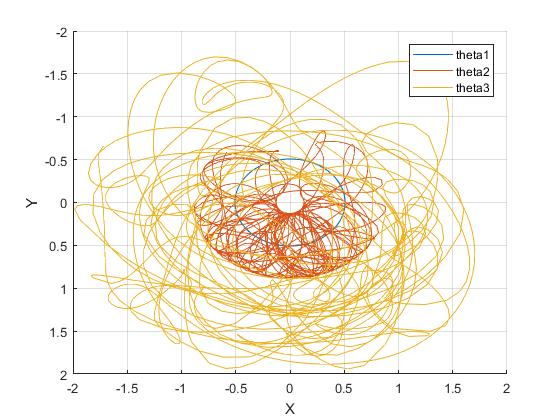
\includegraphics[width=1\linewidth]{path2.jpg}
\caption{Plot of Motion of Triple-Pendulum}\label{fig:path2}
\end{subfigure}
\caption{Motion of Triple-Pendulum for t = 0 to t = 20 sec with changed parameters}\label{fig:image4}
\end{figure}

\begin{figure}[H]
\centering
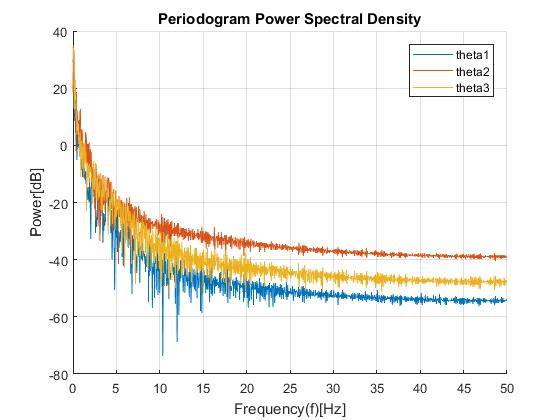
\includegraphics[width=10cm]{p2.jpg}
\caption{Periodogram Plot for ${\theta}$ }\label{fig:p2}
\end{figure}

\begin{figure}[H]
\begin{subfigure}{0.5\textwidth}
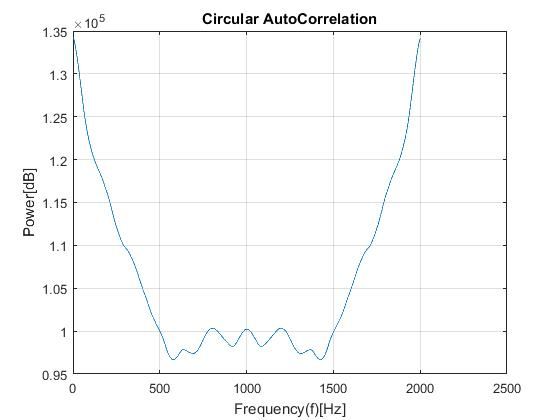
\includegraphics[width=1\linewidth]{cirauto2.jpg}
\caption{Plot of Circular Auto-Correlation for ${\theta_{1}}$}\label{fig:cirauto2}
\end{subfigure}
\begin{subfigure}{0.5\textwidth}
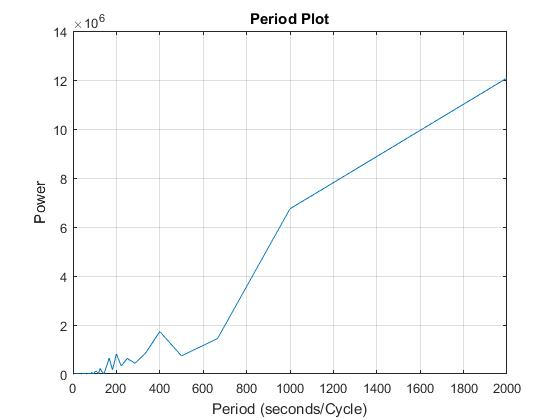
\includegraphics[width=1\linewidth]{pp2.jpg}
\caption{Plot of Periodicity for ${\theta_{1}}$}\label{fig:pp2}
\end{subfigure}
\caption{Periodic Properties of ${\theta_{1}}$}\label{fig:image5}
\end{figure}

Thus, it is evident that changing the parameters of the system can result result different nature of motion which may produce more chaotic behavior.

The obtained values from the periodicity test and the plots generated involving {\em Circular Auto-correlation} and {\em Periodicity} clearly validates the test and differentiates the parameters and initial values which leads to periodic nature of the motion and those which lead to non-periodic nature of the motion.

Our approach is to convert the plain-text into binary format and map the value to an instance in the triple-pendulum motion simulated within a specific duration of time for a particular set of parameters and initial conditions which acts as the key. Another deterministic bijective function can also be used on the mapped value to give double encryption to the plain-text.

\begin{figure}[H]
\centering
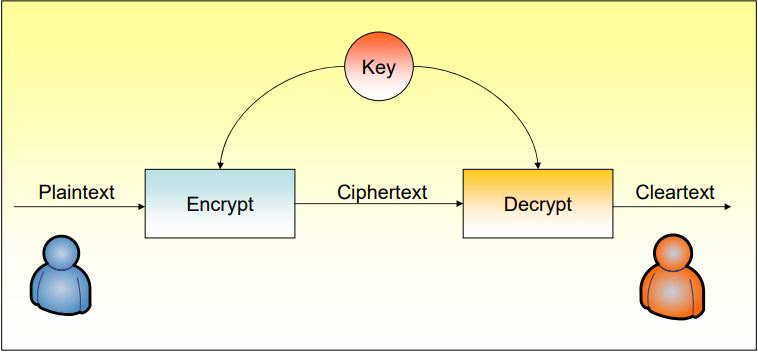
\includegraphics[width=10cm]{crypto.jpg}
\caption{Working Principle of a Cryptosystem}\label{fig:crypto}
\end{figure}

On the decryption module, the second mapping function is known and the mapped value can be obtained by function inversion. Next the mapped value is compared with each instance of the motion of the triple-pendulum for the same key and when an approximate match is obtained the corresponding index would refer to the binary converted clear-text. Converting them into characters, the message can be decoded.\\
\begin{figure}[H]
\centering
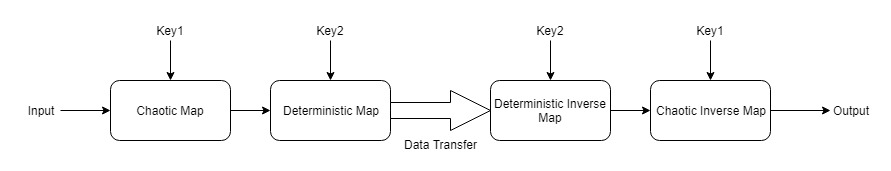
\includegraphics[width=16cm]{DataFlow.jpg}
\caption{Encryption-Decryption Strategy}\label{fig:DataFlow}
\end{figure}

\section{FPGA Implementation}
The complete design is being implemented at Register-Transfer Level (RTL) in {\bf Verilog HDL} and the target device chosen is Digilent Nexys Board with {\bf Xilinx Artix-7 FPGA}. The following diagram shows the implementation plan for the design :
\begin{figure}[H]
\centering
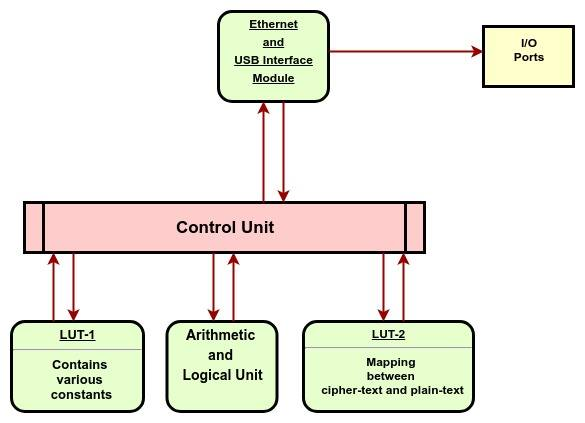
\includegraphics[width=10cm]{fpga_block.jpg}
\caption{Block Diagram of FPGA Implementation}\label{fig:fpga_block}
\end{figure}

1. {\bf Arithmetic and Logical Unit (ALU)} - The ALU uses floating-point arithmetic whose precision can be configured at the time of synthesis. This has been done to enable the study of how security strength varies with arithmetic precision.

2. {\bf Look-Up Table (LUT)} - A fast Look-Up table is to be implemented for storing various constants and the mapping between clear-text and cipher-text.

3. {\bf Ethernet and USB Module} - These are required to enable the device to encrypt or decrypt both a stream of data as well as complete file.

4. {\bf Control Unit} - Essentially a state machine that co-ordinates the operation of all other modules including evaluation of state-variables and transfer of data through USB/Ethernet port.
